\documentclass[a4paper,11pt]{article}
\usepackage{amsmath,amsthm,amsfonts,amssymb,amscd,amstext,vmargin,graphics,graphicx,tabularx,multicol} \usepackage[french]{babel}
\usepackage[utf8]{inputenc}  
\usepackage[T1]{fontenc} 
\usepackage[T1]{fontenc}
\usepackage{amsmath,amssymb}
\usepackage{pstricks-add,tikz,tkz-tab,variations}
\usepackage[autolanguage,np]{numprint} 
\usepackage{color}
\usepackage{ulem}

\setmarginsrb{1.5cm}{0.5cm}{1cm}{0.5cm}{0cm}{0cm}{0cm}{0cm} %Gauche, haut, droite, haut
\newcounter{numexo}
\newcommand{\exo}[1]{\stepcounter{numexo}\noindent{\bf Exercice~\thenumexo} : \marginpar{\hfill /#1}}
\reversemarginpar


\newcounter{enumtabi}
\newcounter{enumtaba}
\newcommand{\q}{\stepcounter{enumtabi} \theenumtabi.  }
\newcommand{\qa}{\stepcounter{enumtaba} (\alph{enumtaba}) }
\newcommand{\initq}{\setcounter{enumtabi}{0}}
\newcommand{\initqa}{\setcounter{enumtaba}{0}}

\newcommand{\be}{\begin{enumerate}}
\newcommand{\ee}{\end{enumerate}}
\newcommand{\bi}{\begin{itemize}}
\newcommand{\ei}{\end{itemize}}
\newcommand{\bp}{\begin{pspicture*}}
\newcommand{\ep}{\end{pspicture*}}
\newcommand{\bt}{\begin{tabular}}
\newcommand{\et}{\end{tabular}}
\renewcommand{\tabularxcolumn}[1]{>{\centering}m{#1}} %(colonne m{} centrée, au lieu de p par défault) 
\newcommand{\tnl}{\tabularnewline}

\newcommand{\trait}{\noindent \rule{\linewidth}{0.2mm}}
\newcommand{\hs}[1]{\hspace{#1}}
\newcommand{\vs}[1]{\vspace{#1}}

\newcommand{\N}{\mathbb{N}}
\newcommand{\Z}{\mathbb{Z}}
\newcommand{\R}{\mathbb{R}}
\newcommand{\C}{\mathbb{C}}
\newcommand{\Dcal}{\mathcal{D}}
\newcommand{\Ccal}{\mathcal{C}}
\newcommand{\mc}{\mathcal}

\newcommand{\vect}[1]{\overrightarrow{#1}}
\newcommand{\ds}{\displaystyle}
\newcommand{\eq}{\quad \Leftrightarrow \quad}
\newcommand{\vecti}{\vec{\imath}}
\newcommand{\vectj}{\vec{\jmath}}
\newcommand{\Oij}{(O;\vec{\imath}, \vec{\jmath})}
\newcommand{\OIJ}{(O;I,J)}

\newcommand{\bmul}[1]{\begin{multicols}{#1}}
\newcommand{\emul}{\end{multicols}}


\newcommand{\reponse}[1][1]{%
\multido{}{#1}{\makebox[\linewidth]{\rule[0pt]{0pt}{20pt}\dotfill}
}}

\newcommand{\titre}[5] 
% #1: titre #2: haut gauche #3: bas gauche #4: haut droite #5: bas droite
{
\noindent #2 \hfill #4 \\
#3 \hfill #5

\vspace{-1.6cm}

\begin{center}\rule{6cm}{0.5mm}\end{center}
\vspace{0.2cm}
\begin{center}{\large{\textbf{#1}}}\end{center}
\begin{center}\rule{6cm}{0.5mm}\end{center}
}



\begin{document}
\pagestyle{empty}
\titre{Contrôle 3 : Transformations et homothétie}{Nom}{Prénom}{Date}{Classe}





\exo{5.5}
On appelle $T_{1}$ la figure représentée par le polygone ABCDEFG. \\
\initq \q Recopier la figure suivante \textbf{au centre de votre copie} à l'aide des carreaux.\\


\includegraphics[scale=0.9]{exotranf3.eps} 


\q Construire ensuite :\\
\qa l'image $T_{2}$ de T par la symétrie axiale d'axe (ED) ;\\
\qa l'image $T_{3}$ de T par la symétrie centrale de centre B ;\\
\qa l'image $T_{4}$ de T par la rotation de  centre  F,  d'angle  90\degre,  dans  le sens inverse des aiguilles d'une montre;\\
\qa l'image $T_{5}$ de T par la translation qui transforme le point B en F.\\



\exo{1} Ci-dessous, on retrouve plusieurs figures avec leurs images créées par homothétie. \\
Les images sont notées avec *.\\
Trouver \textbf{le centre et le rapport} de chacune de ces homothéties.



\includegraphics[scale=0.9]{centrehomo.eps} \hspace*{1.5cm} 
\includegraphics[scale=0.9]{centrehomo2.eps} \\


\exo{2}

\noindent \initq \q Placer le point B' image du point B par l'homothétie de centre O et de rapport k = 7.\\
\q Placer le point A' image du point A par l'homothétie de centre O et de rapport k = 0,6.\\

 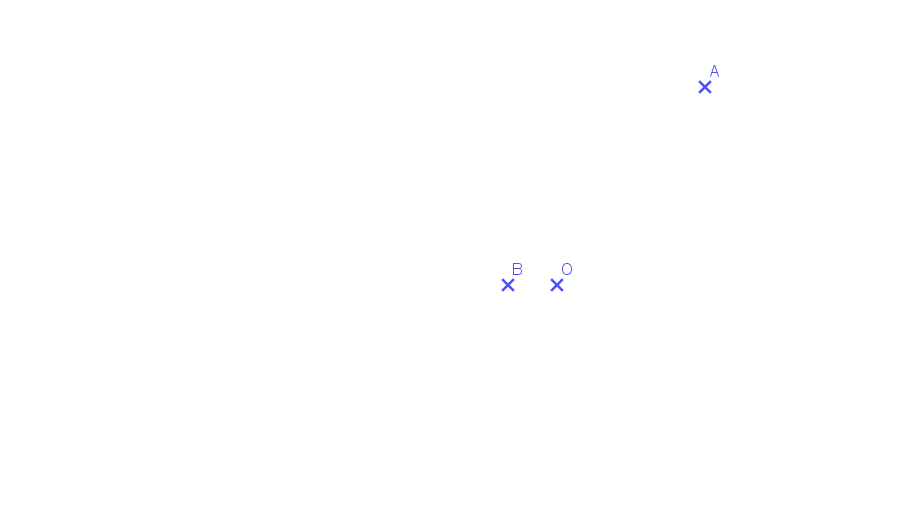
\includegraphics[scale=1.1]{exohomo1.eps} 





\exo{4} Construire :\\
\initqa \qa B' l'image de BOB par l'homothétie de centre J et de rapport $k= -1$\\
\qa B'' l'image de BOB par l'homothétie de centre K et de rapport $k=-0.75$\\

\vspace*{2cm}

\includegraphics[scale=0.8]{exotransfbob.eps} 




\exo{3.5} \initq \q Construire $F_{2}$ l'image de la figure $F_{1}$ par l'homothétie de centre F et de rapport $k=\dfrac{1}{2}$.


\begin{flushleft}
\includegraphics[scale=0.7]{exotranfpositif.eps} 
\end{flushleft}

\q L'aire de la figure $F_{1}$ est de 48 $cm^{2}$. Quelle est l'aire de son image $F_{2}$ par l'homothétie de centre F et de rapport $k=\dfrac{1}{2}$ ? Justifier votre réponse.\\

\newpage

\exo{4.5}

Les droites (AE) et (OC) sont sécantes en B. \\
Le triangle ABC est l'image du triangle OBE par une homothétie.

\begin{center}
\includegraphics[scale=1]{homorapport.eps}
\end{center} 



\initq 
\noindent \q Quel est le centre de cette homothétie?\\
\q Quel est le rapport de cette homothétie? Justifier votre réponse.\\
\q Calculer la longueur du segment [BE] et du segment [OE]. Justifier votre réponse.\\
\q Que peut-on dire des droites (AC) et (OE) ? Justifier votre réponse.\\




\end{document}
